\documentclass[
../../Software_Engineering_Summary.tex,
]
{subfiles}

\externaldocument[ext:]{../../Software_Engineering_Summary.tex}
% Set Graphics Path, so pictures load correctly
\graphicspath{{../../}}

\begin{document}
\section{Domain Modeling}
Domain modeling is a method for identifying the relative concepts and tasks of a domain. 
It is used to fix the terminology and the fundamental activities of the domain.

\begin{defbox}
    [Domain Model]
    \begin{itemize}
        \item Goal: 
        \begin{itemize}
            \item Decompose domain into concepts or objects
            \item Represent the real word (as defined by requirements specifications)
        \end{itemize}
        \item Creation:
        \begin{itemize}
            \item Identify a set of conceptual classes and fundamental actions
            \item Completed iteratively, forms basis or software design
        \end{itemize}
        \item Synonyms:
        \begin{itemize}
            \item Conceptual Model, domain object model, analysis object model
        \end{itemize}
    \end{itemize}
\end{defbox}

\begin{defbox}
    [Conceptual Classes]
    \begin{itemize}
        \item Represents ideas, things or objects in the domain
        \item Attributes:
        \begin{itemize}
            \item Name or Symbol representing the class
            \item Intention
            \item Extension (contains domain elements)
        \end{itemize}
    \end{itemize}
\end{defbox}

\subsection{Visualization of Domain Models}
Domain Models are visualized using \textbf{UML Class Diagrams} with suitable restrictions to emphasize domain modeling:
\begin{itemize}
    \item Only domain objects and conceptual classes
    \item Only associations, no aggregation, no composition
    \item Classes may have attributes but no operations
\end{itemize}

\begin{figure}
    [htp]
    \begin{minipage}
        [t]{0.5\textwidth}
        \centering
        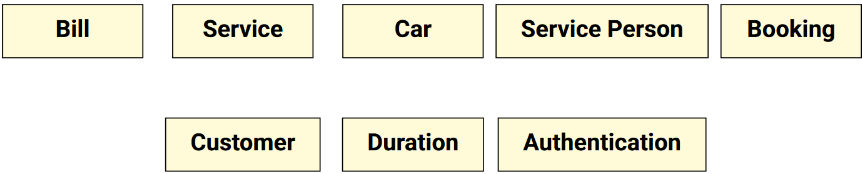
\includegraphics[width=0.95\textwidth]{Pics/04/FirstClassModel.png}
        \caption{Example of Conceptional class (Car sharing)}
    \end{minipage}
    \hfill
    \begin{minipage}
        [t]{0.5\textwidth}
        \centering
        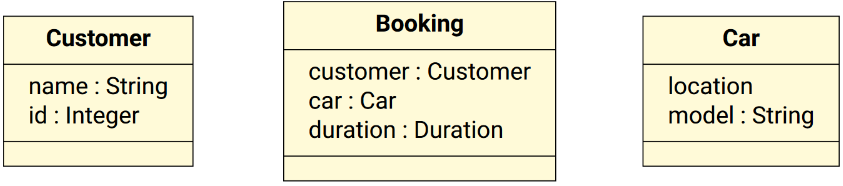
\includegraphics[width=0.95\textwidth]{Pics/04/ConceptualClass.png}
        \caption{Example of conceptual classes with attributes (domain objects)}
    \end{minipage}
\end{figure}

Hereby an objext is defined as an individual thing with a state and relations to other objects.

\begin{defbox}
    [UML Class Elements and Conventions]
    \begin{itemize}
        \item Class Name: Always starts with an upper case letter
        \item Attributes:
        \begin{itemize}
            \item Name: starts with a lower case letter
            \item Type: Pre-defined type or other domain model class (can be omitted)
        \end{itemize}
        \item Derived Attribute:
        \begin{itemize}
            \item Name: prefixed by a slash, followed by a lower case letter
            \item Describes a value computable from existing information
        \end{itemize}
    \end{itemize}
\end{defbox}


\begin{defbox}
    [UML Associations / Relations]
    An association is a relation among classes. It consists of the following:
    \begin{itemize}
        \item Name: (optional) Should be done according to the \textbf{Class name-verb phrase-Class name} format:
        \begin{itemize}
            \item \color{teal}Player-\color{magenta}Stands-on\color{teal}-Square
            \item \color{teal}Sale-\color{magenta}Paid-by\color{teal}-CashPayment
            \item \color{teal}Customer-\color{magenta}Traveled-by\color{teal}-Vehicle
        \end{itemize}
        \item Two Roles (associations):
        \begin{itemize}
            \item Name: Defaults to class name in lowercase
            \item Multiplicity: Defaults to 1. \\ Possible: * (arbitrary/all) and a..b (Range, upper bound inclusive)
            \item Navigability: Defaults to bidirectional, not used for conceptual classe.
        \end{itemize}
    \end{itemize}
    \begin{minipage}
        [m]{0.6\textwidth}
        \centering
        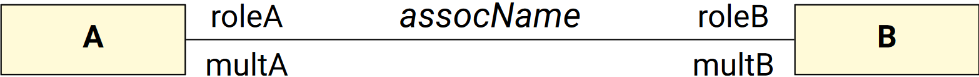
\includegraphics[width=0.95\textwidth]{Pics/04/UMLClassesAssociations.png}
    \end{minipage}
    \hfill
    \begin{minipage}
        [m]{0.4\textwidth}
        \centering
        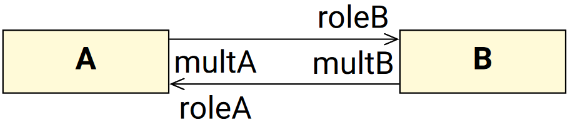
\includegraphics[width=0.95\textwidth]{Pics/04/UMLClassesDirectional.png}
    \end{minipage}

    Associations should be included in the domain model if the knowledge of the relation needs to be preserved. For example: The relation between a bill and its entries needs to be preserved. However the relation between a user and their recent searches is not necessarily important.
\end{defbox}
\begin{figure}
    [htp]
    \centering
    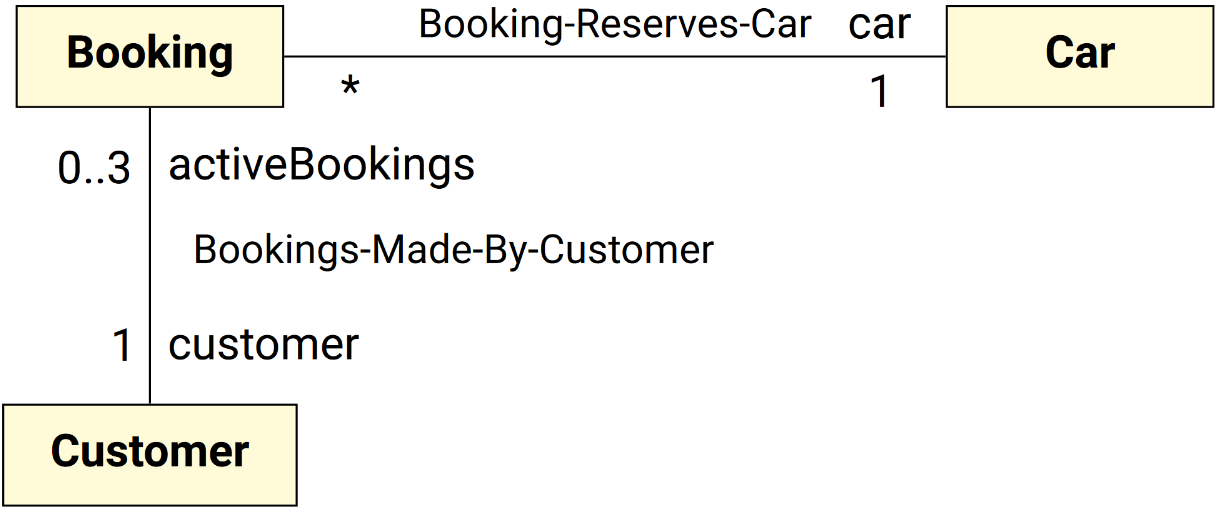
\includegraphics[scale = 0.35]{Pics/04/UMLClassAssociationExample.png}
    \caption{Example of UML Class Association}
\end{figure}



\begin{defbox}
    [Class Generalizations]
    Multiple classes can be comprised of multiple subclasses:
    \centering
    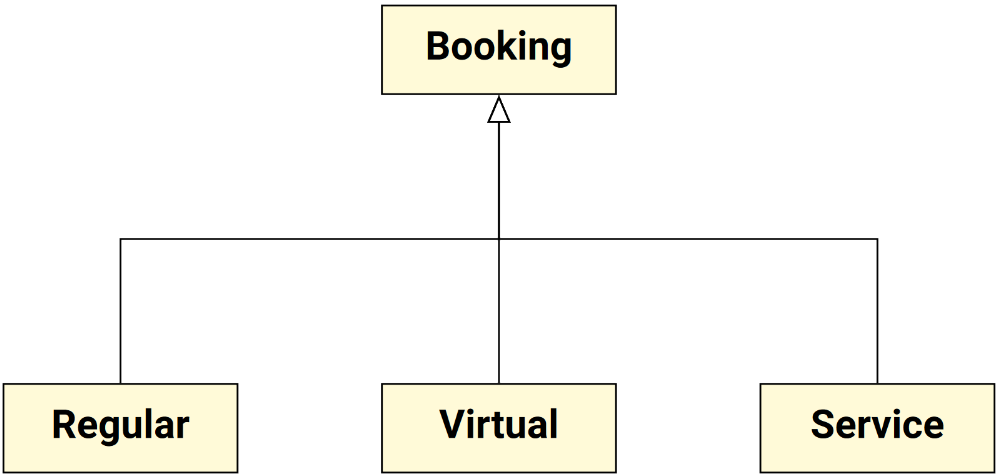
\includegraphics[scale = 0.4]{Pics/04/UMLClassGeneralizations.png}
\end{defbox}

\subsection{Eliciation of Domain Models}
\begin{defbox}
    [Workflow]
    \begin{enumerate}
        \item Find the conceptual classes
        \\ Strategies:
        \begin{itemize}
            \item Re-Use or modify existing model
            \item Use a category list
            \item Identify noun phrases
        \end{itemize}
        \item Draw elicited concepts as classes in a UML class diagram
        \item Add attributes
        \item Add associations
    \end{enumerate}
\end{defbox}

\subsubsection{Re-Using Existing Models}
\begin{figure}[htp]
    \centering
    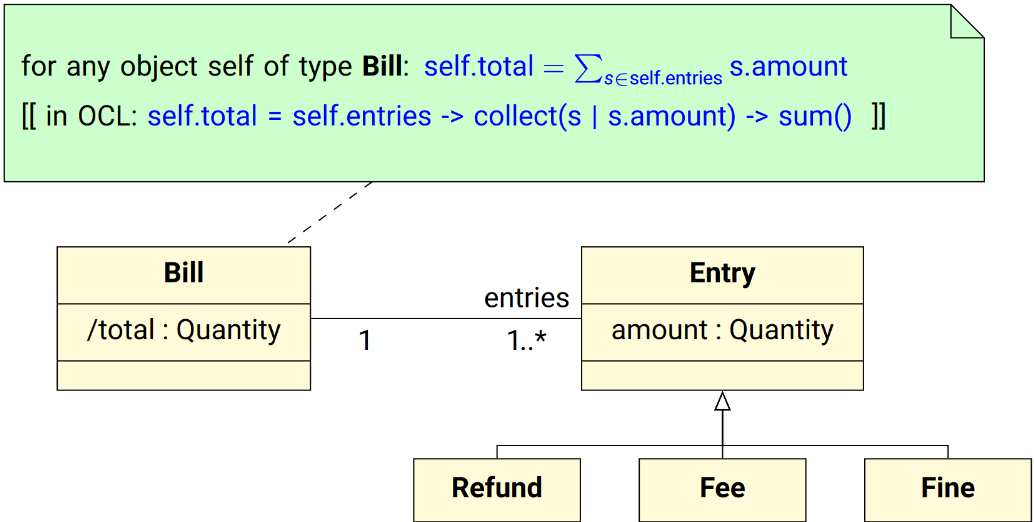
\includegraphics[scale=0.4]{Pics/04/ReUsingConceptualClasses.png}
\end{figure}

\subsubsection{List of Conceptual Classes Categories}
Some Categories:
\begin{itemize}
    \item Physical objects
    \item Specifications of things
    \item Locations
    \item Events
    \item Transactions
    \item etc.
\end{itemize}
\begin{figure}[htp]
    \centering
    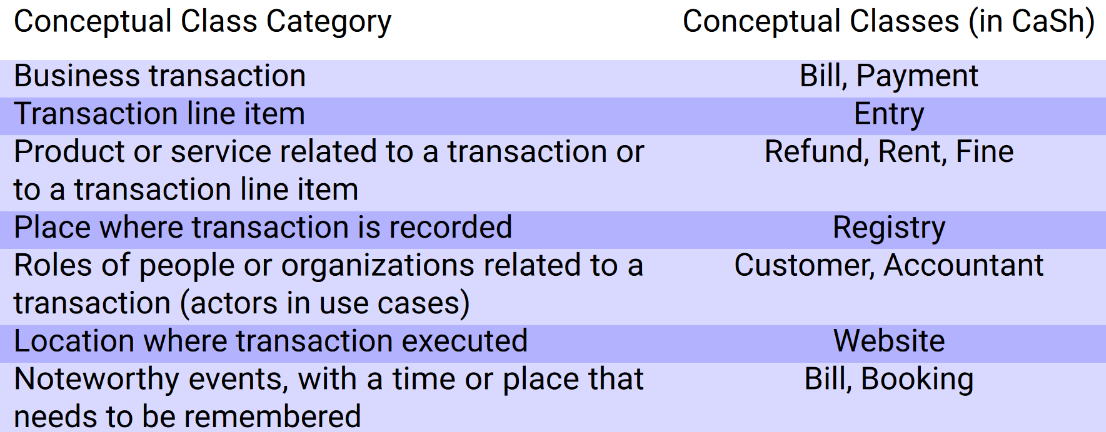
\includegraphics[scale=0.5]{Pics/04/CategoryListExample.png}
\end{figure}

\newpage
\subsubsection{Noun Identification}
Workflow:
\begin{enumerate}
    \item Identify nouns and noun phrases in textual description (Use Cases for example) of domain
    \item Consider them as a candidate for a conceptual class or attribute
\end{enumerate}

Criteria for inclusion of conceptual classes:
\begin{itemize}
    \item Must carry information not available/computable from other sources
    \item Must have specific semantic in relation to the business
\end{itemize}

Can only be partially automated due to the ambiguity of natural language

\subsection{Description Classes}
A description class contains information that describes an entity. For example, a description class for a car would contain information about the car's make, model, color, etc.

A description class should be added to the model if: 
\begin{itemize}
    \item Information about the entity is required, regardless of whether an instance of the entity even exists.
    \item Deleting an instance of the entity would result in loss of information.
    \item Redundant or duplicate information is reduced
\end{itemize}

\begin{defbox}
    [Class or Attribute]
    When deciding if a piece of information should be included as an attribute or a class:
    If notion C is not considered:
    \begin{itemize}
        \item Number
        \item Text
        \item Date
    \end{itemize}
    that usually indicates that it should be a \textbf{class}.
    \begin{center}
        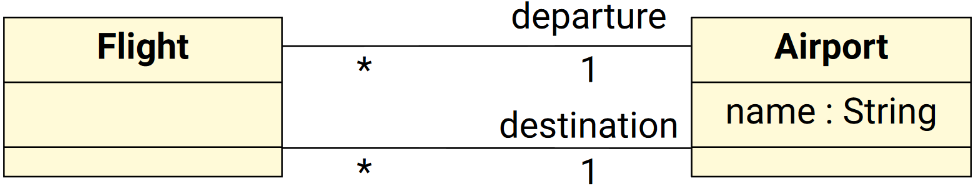
\includegraphics[width=0.65\textwidth]{Pics/04/ClassVsAttributeExample.png}
        \captionof*{figure}{When considering the destination of a flight, it makes more sense to put that information into a class Airport, instead of making it an attribute of flight. Also allows for better alotment of additional info.}
    \end{center}
\end{defbox}

\begin{defbox}
    [When to use Attributes or Associations]
    \begin{itemize}
        \item Attributes should always describe primitive datatypes:
        \begin{itemize}
            \item Boolean, Integer, Character, String\dots
            \item Dates, Address, Colors, Phone Numbers\dots
        \end{itemize}
        \item Quantities may be modelled as classes to attach units:
        \begin{itemize}
            \item currency: EUR, USD, CAD\dots
            \item distance: meters, miles, millimeters\dots
        \end{itemize}
        \item Relations between conceptual classes are always associations
    \end{itemize}
\end{defbox}

\newpage
\subsubsection{Refining the model}
Initially it is very convenient to type attributes with Strings. It is a generic type that avoids premature decision. Later on it can be refined into a description class:
\begin{figure}[htp]
    \centering
    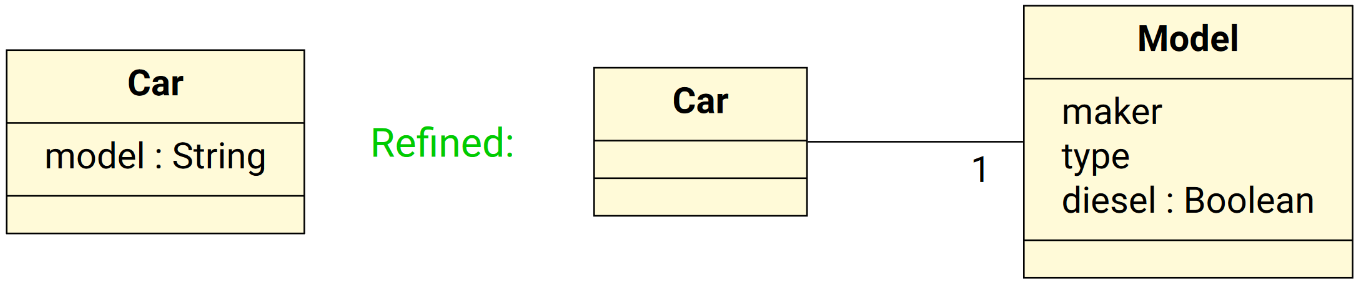
\includegraphics[scale=0.5]{Pics/04/RefiningModelTypes.png}
\end{figure}

Obviously a string can only be refined if it actually contains more information that can be shown differently. 

In general, the domain model serves as an inspiration for the design model later on.
\begin{figure}
    [htp]
    \centering
    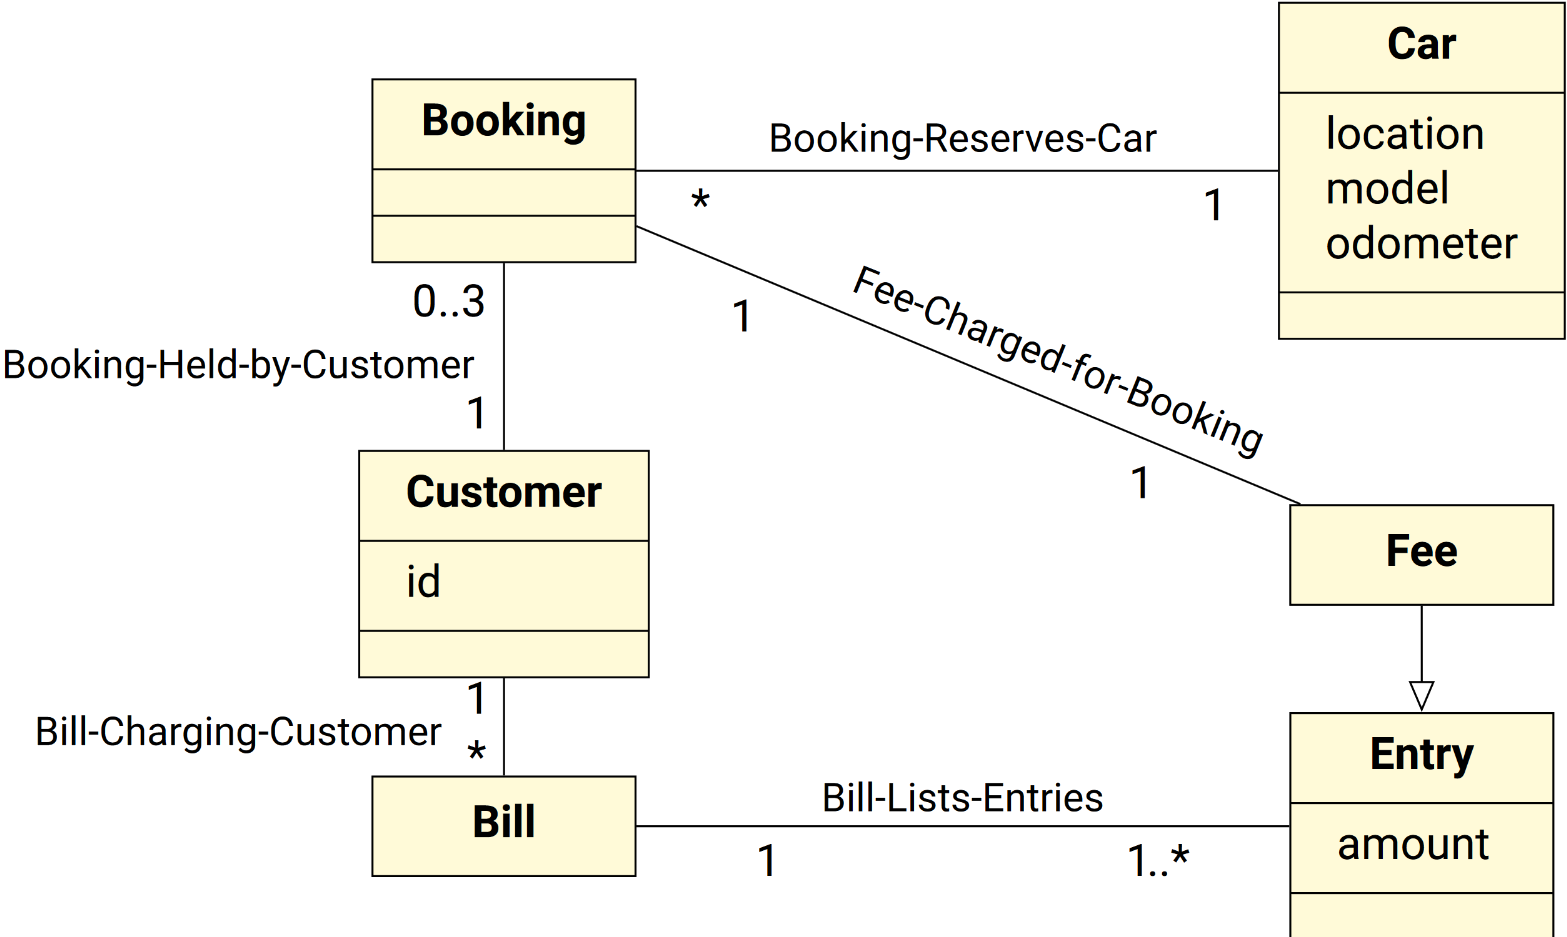
\includegraphics[scale= 0.4]{Pics/04/DomainModelExample.png}
    \caption{An example Domain Model}
\end{figure}

\newpage
\subsection{Behavioural Domain Modelling}
Class Diagrams only model static aspects such as classes, objects, attributes, associations and functions. 

What we are missing are the behaviours, the sequence of actions and how they change the state of the system and under which condition.

These behaviours can be displayed as UML State Machines Diagrams.

\begin{defbox}
    [UML State Machine Diagrams]
    \begin{center}
        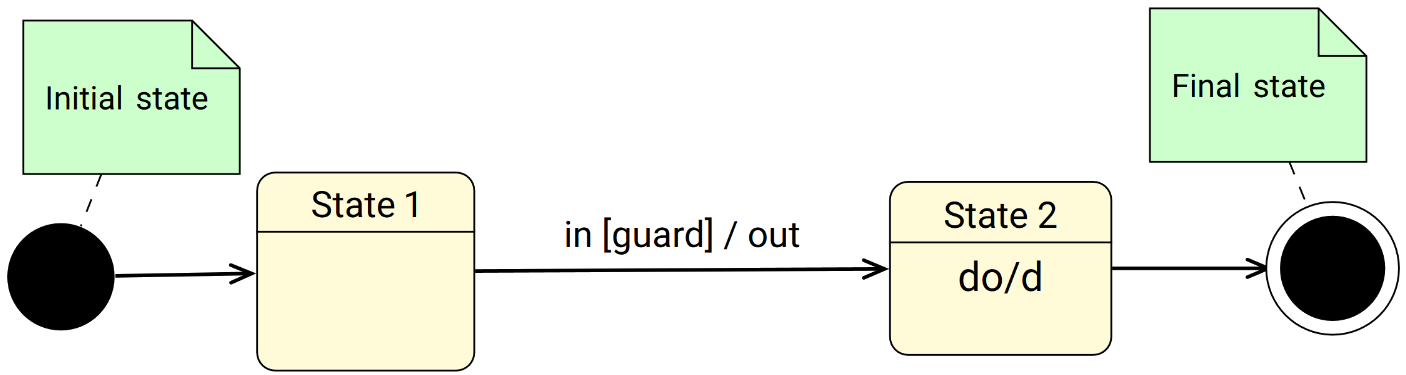
\includegraphics[scale=0.5]{Pics/04/UMLStateMachineDiagrams.png}
    \end{center}
    This can be read as: \textit{When in State 1, if input in is observed and guard is true, then output out happens and current state becomes state 2. In state 2 perform the (interruptible) action d}.

    So in General UML State Machine Diagrams show States and their conditions for transitioning as in- and outputs and guards.
\end{defbox}

\begin{defbox}
    [Basic States]
    \begin{center}
        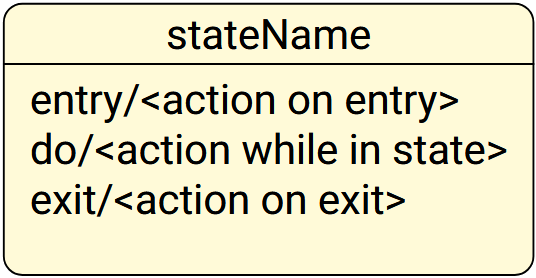
\includegraphics[scale=0.3]{Pics/04/BehaviourBasicStates.png}
    \end{center}
    States consist of the following:
    \begin{itemize}
        \item Name: Short description of what the state represents
        \item Actions: Executed Operations
        \begin{itemize}
            \item Entry: Action performed on state entry
            \item Do: Action performed while in state (until terminated or state is left)
            \item Exit: Action performed on state exit
        \end{itemize}
    \end{itemize}
\end{defbox}

\begin{defbox}
    [Special States]
    \begin{center}
        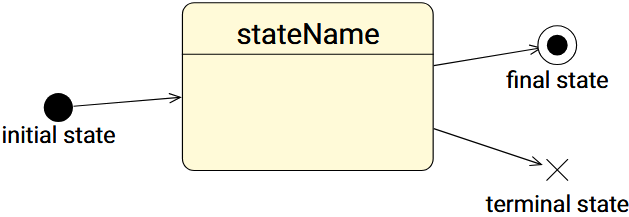
\includegraphics[scale=0.5]{Pics/04/BehaviourSpecialStates.png}
    \end{center}
    There are some special states:
    \begin{itemize}
        \item Initial State: Has a single transition to first entered state \\
        May be labeled by object creation event
        \item Final State: Indicates completion of scenario
        \item Terminal State: Completion and executing object destroyed
    \end{itemize}
\end{defbox}

\begin{defbox}
    [Transitions]
    \begin{center}
        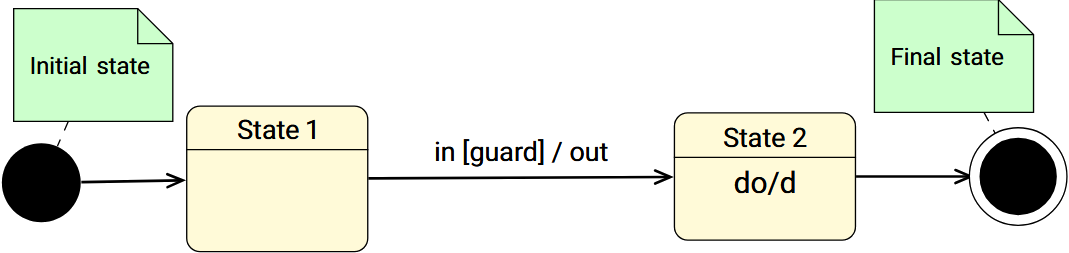
\includegraphics[scale=0.4]{Pics/04/BehaviourTransitions.png}
    \end{center}
    A transition label is usually in the format \textbf{input? [guard]? / output?}. Hereby all components are optional (therfore ?).
    \begin{itemize}
        \item Input (Trigger) events are observations:
        \begin{itemize}
            \item call event (start of operation)
            \item time event (e.g. time spent in a state)
            \item change event (value of attribute has changed)
        \end{itemize}
        \item Guard is a boolean expression (for example: if input == value)
        \item Output (action) is an operation
    \end{itemize}
\end{defbox}

In general, the purpose of state machine diagrams are:
\begin{itemize}
    \item Capturing action sequences of a use case
    \item Combine related use cases
    \item Clarify the states of an object
    \item Clarify protocols
    \item Validate the domain model
    \item Complete the domain model (properties, actions)
    \item Model \textbf{only} non-trivial behaviour
\end{itemize}

\begin{figure}
    [htp]
    \centering
    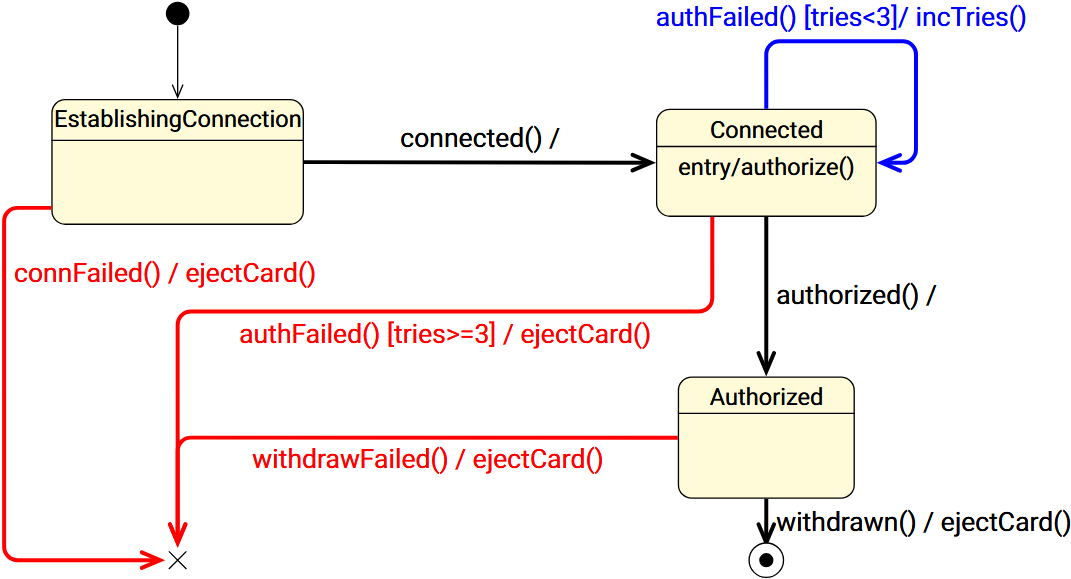
\includegraphics[scale=0.5]{Pics/04/StateMachineDiagramExample.png}
    \caption{An example State Machine Diagram}
\end{figure}
\end{document}
